\documentclass{mwrep}

% Polskie znaki
\usepackage{polski}
\usepackage[utf8]{inputenc}
\usepackage[T1]{fontenc}
\usepackage{lmodern}
\usepackage{indentfirst}

% Strona tytułowa
\usepackage{pgfplots}
\usepackage{siunitx}
\usepackage{paracol}

% Pływające obrazki
\usepackage{float}
\usepackage{svg}
\usepackage{graphicx}

% table of contents refs
\usepackage{hyperref}
\usepackage{cleveref}
\usepackage{booktabs}
\usepackage{listings}


\SendSettingsToPgf
\title{\bf Sprawozdanie z bloku drugiego \vskip 0.1cm}
\author{Konrad Winnicki \\ Jakub Sikora}
\date{\today}
\pgfplotsset{compat=1.15}	
\begin{document}

\makeatletter
\renewcommand{\maketitle}{\begin{titlepage}
		\begin{center}{
				\LARGE {\bf Politechnika Warszawska}}\\
            \vspace{0.4cm}
            \leftskip-0.9cm
            {\LARGE {\bf \mbox{Wydział Elektroniki i Technik Informacyjnych}}}\\
            \vspace{0.2cm}
            {\LARGE {\bf \mbox{Instytut Automatyki i Informatyki Stosowanej}}}\\
            
            \vspace{5cm}
            \leftskip-0.5cm
			{\bf \Huge \mbox{Sterowanie i symulacja robotów} \vskip 0.1cm}
		\end{center}
		\vspace{0.1cm}

		\begin{center}
			{\bf \LARGE \@title}
		\end{center}

		\vspace{10cm}
		\begin{paracol}{2}
			\addtocontents{toc}{\protect\setcounter{tocdepth}{1}}
			\subsection*{Zespół:}
			\bf{ \Large{ \noindent\@author \par}}
			\addtocontents{toc}{\protect\setcounter{tocdepth}{2}}

			\switchcolumn \addtocontents{toc}{\protect\setcounter{tocdepth}{1}}
			\subsection*{Prowadzący:}
			\bf{\Large{\noindent mgr. inż. Wojciech \\ Dudek}}
			\addtocontents{toc}{\protect\setcounter{tocdepth}{2}}

		\end{paracol}
		\vspace*{\stretch{6}}
		\begin{center}
			\bf{\large{Warszawa, \@date\vskip 0.1cm}}
		\end{center}
	\end{titlepage}
}
\makeatother
\maketitle

\tableofcontents

\chapter{Laboratorium 1}
\label{lab1}

\section{Znalezione błędy w funkcjonowaniu systemu robota}
\label{lab1_errors}
W trakcie zajęć po wprowadzeniu przez prowadzącego kilku modyfikacji,
system robota przestał działać poprawnie. Po zadaniu robotowi prędkości, 
robot zatrzymywał się i ruszał w bardzo dziwny i niezrozumiały sposób.
Naszym zadaniem było zlokalizować usterki za pomocą narzędzi
systemu ROS. 

\subsection{Wykorzystane narzędzia}
\label{lab1_errors_tools}
Do zdiagnozowania usterki systemu wykorzystaliśmy następujące narzędzia.

\subsubsection{\texttt{rqt\_{}graph}}
Narzędzie \texttt{rqt\_{}graph} służy do wizualizacji struktury systemu. Pozwala na
śledzenie topologii komunikacji pomiędzy poszczególnymi węzłami. Za pomocą tego narzędzia
mogliśmy sprawdzić czy zaburzona została komunikacja pomiędzy węzłami oraz czy
nie dodano nowego węzła wprowadzającego zaburzenia.

\subsubsection{\texttt{rqt\_{}tf\_{}tree}}
Narzędzie \texttt{rqt\_{}tf\_{}tree} pozwala na wizualizację drzewa transformacji 
w systemie robota. Program pozwolił nam na sprawdzenie czy publikowane są wszystkie
transformację w systemie, pozwalające na poprawne wykonywanie obliczeń w systemie.

\subsubsection{\texttt{rostopic}}
Program \texttt{rostopic} jest narzędziem do sprawdzenia informacji
na temat ROS Topiców. Narzędzie to pozwala na wypisywanie wiadomości 
nadawanych na zadanym kanale, znajdywania wszystkich topiców czy publikowanie
nowych wiadomości.

\subsubsection{\texttt{rqt\_{}plot}}
Narzędzie \texttt{rqt\_{}plot} pozwala na wizualizację danych z wiadomości
na kolorowych wykresach. Zwykle używane jako pierwsze narzędzie po które sięgamy 
w trakcie pracy z systemem, to jednak w zadaniu lokalizacji usterki okazał się 
bezużyteczny. 

\subsection{Zlokalizowane usterki}
\label{lab1_errors_faults}
Za pomocą \texttt{rqt\_{}tf\_{}tree} udało nam się ustalić że brakuje transformacji z
układu bazy robota do układu wieży. Brak tego przekształcenia nie pozwalał chociażby
na poprawną wizualizację robota w programie \texttt{rviz}. \\
\\
Znacznie poważniejszą usterką wprowadzoną przez prowadzącego było dołączenie do systemu
nowego węzła nadającego na topic \texttt{mux\_{}vel\_{}nav/cmd\_{}vel}. Anonimowy węzeł 
udało nam się zlokalizować za pomocą narzędzia \texttt{rqt\_{}graph}. Po podsłuchaniu 
niechcianego gościa za pomocą polecenia \texttt{rostopic echo} udało nam się ustalić 
że nowy węzeł nadaje zerowe prędkości. Wyjaśnia to zrywane ruchy robota, który najpierw
otrzymywał niezerowe wartości prędkości aby następnie otrzymać polecenie zatrzymania się.

\section{Opis algorytmu interpolacji liniowej}
\label{lab1_interpolation}
Głównym zadaniem do zrealizowania w trakcie laboratorium pierwszego było napisanie węzłów
implementujących względne sterowanie pozycyjne. Należało zrealizować zadanie w dwóch
wariantach. 

\subsection{Interpolacja na podstawie zadawanych prędkości}
\label{lab1_interpolation_noodom}
W pierwszej wersji, interpolowaliśmy punkty wyłacznie za pomocą 
zadawanych prędkości. Węzeł był inicjalizowany w punkcie (0,0,0) a kolejne sterowania
miały być wyznaczane na podstawie domniemanej idealnie zrealizowanej poprzedniej akcji ruchu.\\
\\
\indent{} Zasada działania algorytmu wydaje się banalnie prosta. System sterowania robota cały 
czas zapamiętuje pozycję między akcjami. Po przyjściu nowego polecenia, wyznaczane są 
przemieszczenia o które należy przesunąć robota. Robot najpierw obraca się w stronę zadanego
punktu, następnie jedzie do przodu aż do wyznaczonego miejsca aby ostatecznie obrócić się do 
zadanego kąta obrotu. \\
\\
\indent{} Najciekawszym z punktu widzenia projektowania algorytmu lokomocji wydaje się sposób interpolacji położenia.
Robot poruszając się do przodu zna odległość swoją od położenia zadanego oraz prędkość jaką zadaje
na koła. Korzystając z prostego wzoru na drogę: $$ s = vt $$ możemy w prostu sposób wyznaczyć
przez ile sekund należy jechać/obracać się aby osiągnąć cel. W ten sam sposób interpolowaliśmy
pozycję kątową robota. Korzystając z zależności $$ \alpha = \omega t $$ udało nam się w prosty
sposób uzyskać zadany kąt. Z podanego sposobu korzystamy na początku ruchu aby obrócić robota w
stronę pozycji zadanej i na końcu ruchu aby obrócić robota do docelowego kąta zadanego. \\
\\
\indent{} Korzystająć z tej metody, udało nam się uzyskać wyniki
które można opisać jako wysoko niezadowalające. Nawigacja robotem w ten sposób ma wiele wad.
Jest bardzo niedokładna a błąd bardzo szybko narasta, co czyni wykonywanie złożonych zadań
przemieszczania się niemożliwymi do wykonania. Jedyną zaletą tej metody, jest jej prostota.
Można ją wykorzystać do zgrubnego przemieszczania się robota, w przypadku gdy podłoże 
nie jest śliskie oraz nie jest dostępna informacja z enkoderów.\\
\\
\subsubsection{Implementacja}
Zgodnie z przyjętą konwencją nazewniczą, węzeł wykonujący interpolację na podstawie 
zadawanych prędkości nazwaliśmy \texttt{normalmente\_{}movimiento.py}. Węzeł nasłuchuje 
nowej pozycji zadanej na topicu \texttt{new\_{}pose}, który przyjmuje wiadomości
typu \texttt{turtlesim/Pose}. Polecenie ruchu można wysłać używając przykładowego polecenia:

\begin{center}
    \texttt{rostopic pub /new\_{}pose turtlesim/Pose '{x: 2.0, y: 4.0, theta: 0}'}
\end{center}

po którym węzeł zacznie wysyłać wiadomości typu \texttt{geometry/Twist} na topic 
\texttt{mux\_{}vel\_{}nav/cmd\_{}vel}.

\newpage

\subsection{Interpolacja na podstawie danych odometrii}
\label{lab1_interpolation_odom}
W drugiej wersji węzła, implementowaliśmy interpolację liniową punktów na podstawie 
danych z odometrii. Informacja zwrotna na temat zrealizowanego położenia powinna 
pozwolić na znaczącą poprawę dokładności przemieszczania robota.\\

\indent{} Przed wyjaśnieniem zasady działania algorytmu, należy wyjaśnić czym dokładnie
jest odometria. Najogólniej rzecz biorąć, odometria to dział miernictwa, który zajmuje się 
pomiarem odległości, wykorzystującym czujniki które określają przemieszczenie względem pozycji 
początkowej. \\
\\
\indent{} W przypadku systemu robotycznego Elektron, do dyspozycji mamy dwa rodzaje czujników.
Pierwszym są enkodery umieszczone na kołach robota, które pozwalają na pomiar o ile obróciło się koło,
co przy znanym promieniu powinno z pewną precyzją zwrócić nam przemieszczenie. Drugą możliwością, jest 
zastosowanie czujnika laserowego do pomiaru przemieszczenia względem otoczenia.\\
\\
\indent{} Zasada działania algortymu nie jest specjalnie skomplikowana. Na początku obracamy robota,
aż jego orientacja wynikająca z odometrii będzie zgodna (z zadaną dokładnością) z orientacją wymaganą do jazdy
w kierunku zadanego punktu. Następnie robot jedzie prosto do momentu aż jego pozycja wynikająca
z odometrii będzie zgodna z pozycją zadaną. Ostatecznie, ponownie obracamy robota do zadanej 
orientacji w ten sam sposób w jaki to robiliśmy w pierwszej fazie ruchu.\\
\\
\indent{} Głównym czynnikiem wpływającym na jakość działania węzła jest jakość samego sygnału
z odometrii. W przypadku kierowania się sygnałem pozycji pochodzącym z enkoderów umieszczonych 
na kołach, który jest podatny na błędy z powodu poślizgów i skończonej rozdzielczości samego enkodera,
możemy nie uzyskać dokładnego odwzorowania pozycji zadanej w rzeczywistą pozycję robota. 
W celu poprawienia jakości sygnału z odometrii należy skorzystać z czujnika laserowego LIDAR, który 
zwraca położenie na podstawie przemieszczenia względem otoczenia. 
\subsubsection{Implementacja}
W celu wykonania zadania napisaliśmy skrypt \texttt{odometria\_{}movimiento.py}, który uruchamia węzeł
poruszający robotem z uwzględeniem informacji z odometrii. Podobnie jak w poprzednim zadaniu robot nasłuchuje
nowej pozycji zadanej na temacie \texttt{new\_{}pose}. Dodatkowo, umożliwiliśmy zadawanie nowej pozycji jako 
\texttt{rosservice}. Użytkownik wysyła żądanie przemieszczenia do usługi o nazwie \texttt{stero/go\_{}to\_{}stpt}.
Aby poprawnie wywołać usługę, należy wysłać wiadomość zdefiniowanego przez nas typu \texttt{stero\_{}mobile\_{}init/STPT}.
Węzeł odczytuje informacje z odometrii 
z tematu \texttt{/elektron/mobile\_{}base\_{}controller/odom}. Wiadomości nadawane na tym temacie są typu \texttt{nav/Odometry}.\\
\\
\indent{} Po poprawnym zgłoszeniu żądania przemieszczenia, robot podobnie jak w przypadku poprzedniego węzła, 
wykonuje trzystopniowe przemieszczenie się do pozycji zadanej:\\
\begin{itemize}
	\item Obrót w stronę pozycji zadanej
	\item Ruch po prostej do punktu zadanego
	\item Obrót do zadanej orientacji\\
\end{itemize}

Każda z faz jest wykonywana do momentu gdy pozycja z odometrii będzie zgodna z pozycją zadaną. Ponieważ pozycja jest 
zwracana w pewnych odstępach, przemieszczenia i obroty wykonujemy do momentu aż różnica pozycji odometrii z pozycją
zadaną będzie mniejsza od zadanego poziomu dokładności.

\section{Porównanie odometrii z pozycją referencyjną}
\label{lab1_comparision}
\subsection{Test kwadratu zgodnie z ruchem wskazówek zegara}
\begin{figure}[H]
	\centering
	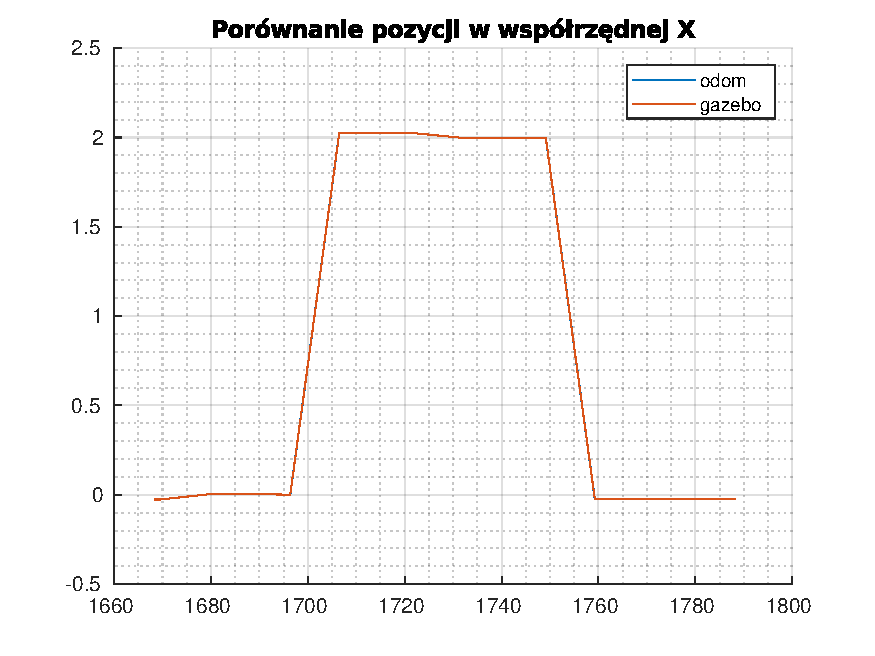
\includegraphics[scale=0.8]{./figures/lab1/lab1xcw.pdf}
	\caption{Pozycja we współrzędnej x osiągana przez robota w trakcie testu kwadratu (zgodnie z ruchem wskazówek zegara)}
\end{figure}

\begin{figure}[H]
	\centering
	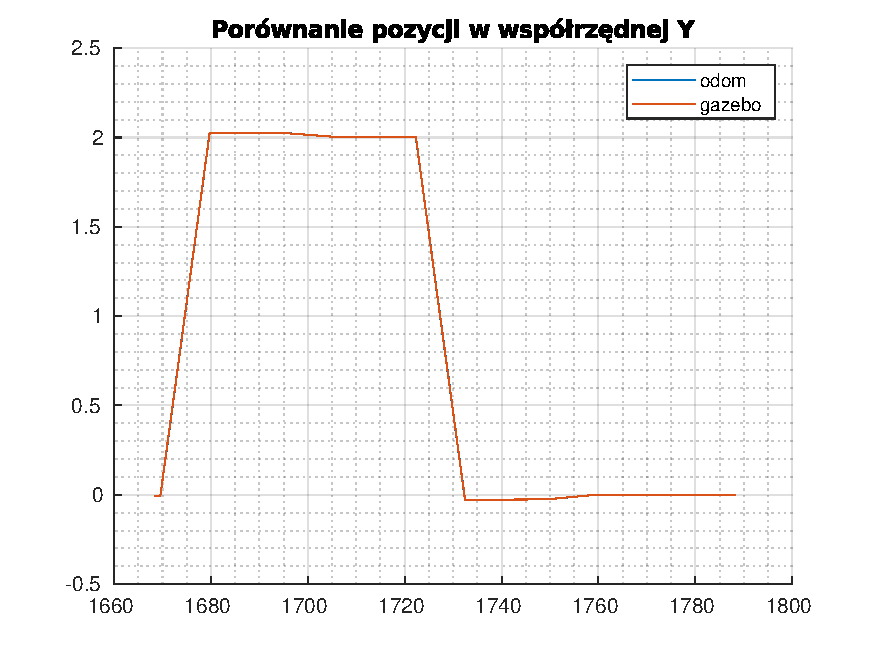
\includegraphics[scale=0.8]{./figures/lab1/lab1ycw.pdf}
	\caption{Pozycja we współrzędnej y osiągana przez robota w trakcie testu kwadratu (zgodnie z ruchem wskazówek zegara)}
\end{figure}
\newpage

\subsection{Test kwadratu przeciwnie do ruchu wskazówek zegara}
\begin{figure}[H]
	\centering
	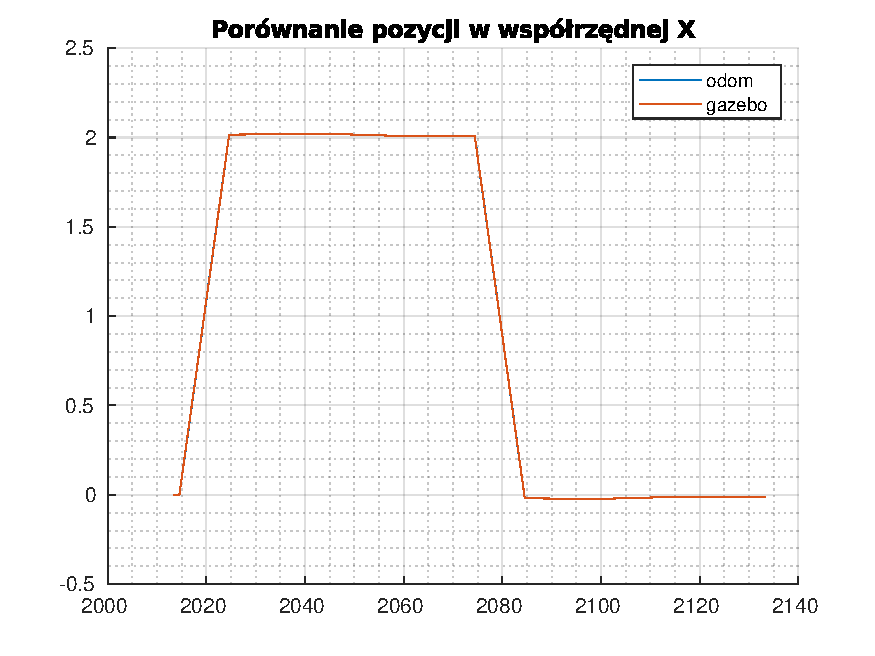
\includegraphics[scale=0.8]{./figures/lab1/lab1xccw.pdf}
	\caption{Pozycja we współrzędnej x osiągana przez robota w trakcie testu kwadratu (przeciwnie do ruchu wskazówek zegara)}
\end{figure}

\begin{figure}[H]
	\centering
	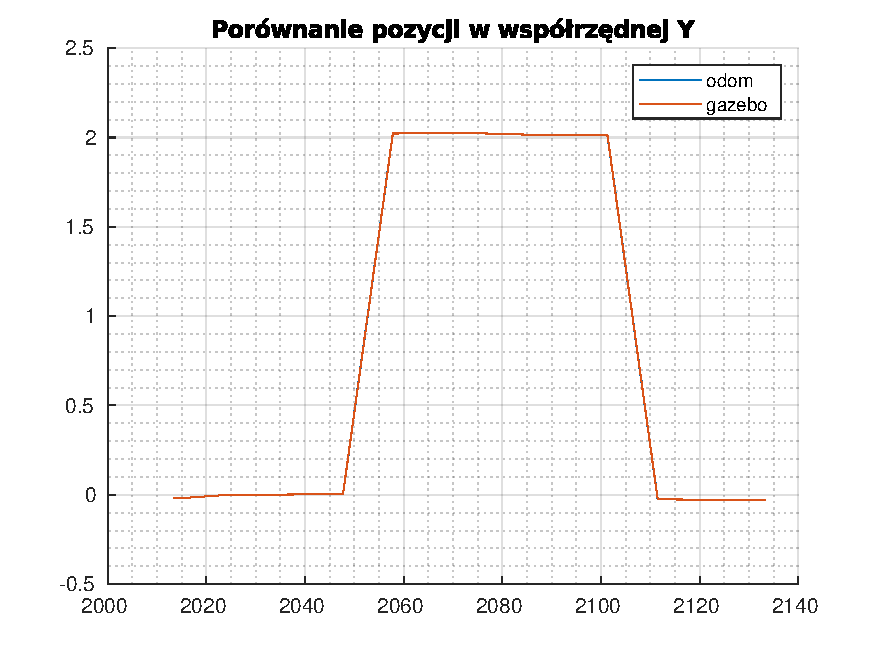
\includegraphics[scale=0.8]{./figures/lab1/lab1yccw.pdf}
	\caption{Pozycja we współrzędnej y osiągana przez robota w trakcie testu kwadratu (przeciwnie do ruchu wskazówek zegara)}
\end{figure}

Pozycja z enkoderów zaskakująco dobrze odwzorowuje aktualną pozycję. Oba pomiary (odom - enkodery, gazebo - pozycja w symulacji)
praktycznie pokrywają się, co pozwala na precyzyjne sterowanie robotem w symulacji. 
Tak dobra jakość sygnału z odometrii spowodowana jest zastosowaniem lepszego sterownika \texttt{diff\_{}drive\_{}controller}s.

\chapter{Projekt 1}
\label{pro1}
W ramach pierwszego projektu w bloku, naszym zadaniem było zebranie danych 
z odometrii z różnych kontrolerów oraz dokonanie ich porównania. Do akwizycji 
danych należało zaimplementować dodatkowy węzeł ROSa.

\section{Struktura oprogramowania stworzonego do zbierania danych}
\label{pro1_struct}

\begin{figure}[H]
	\centering
	\leftskip-0.6cm
	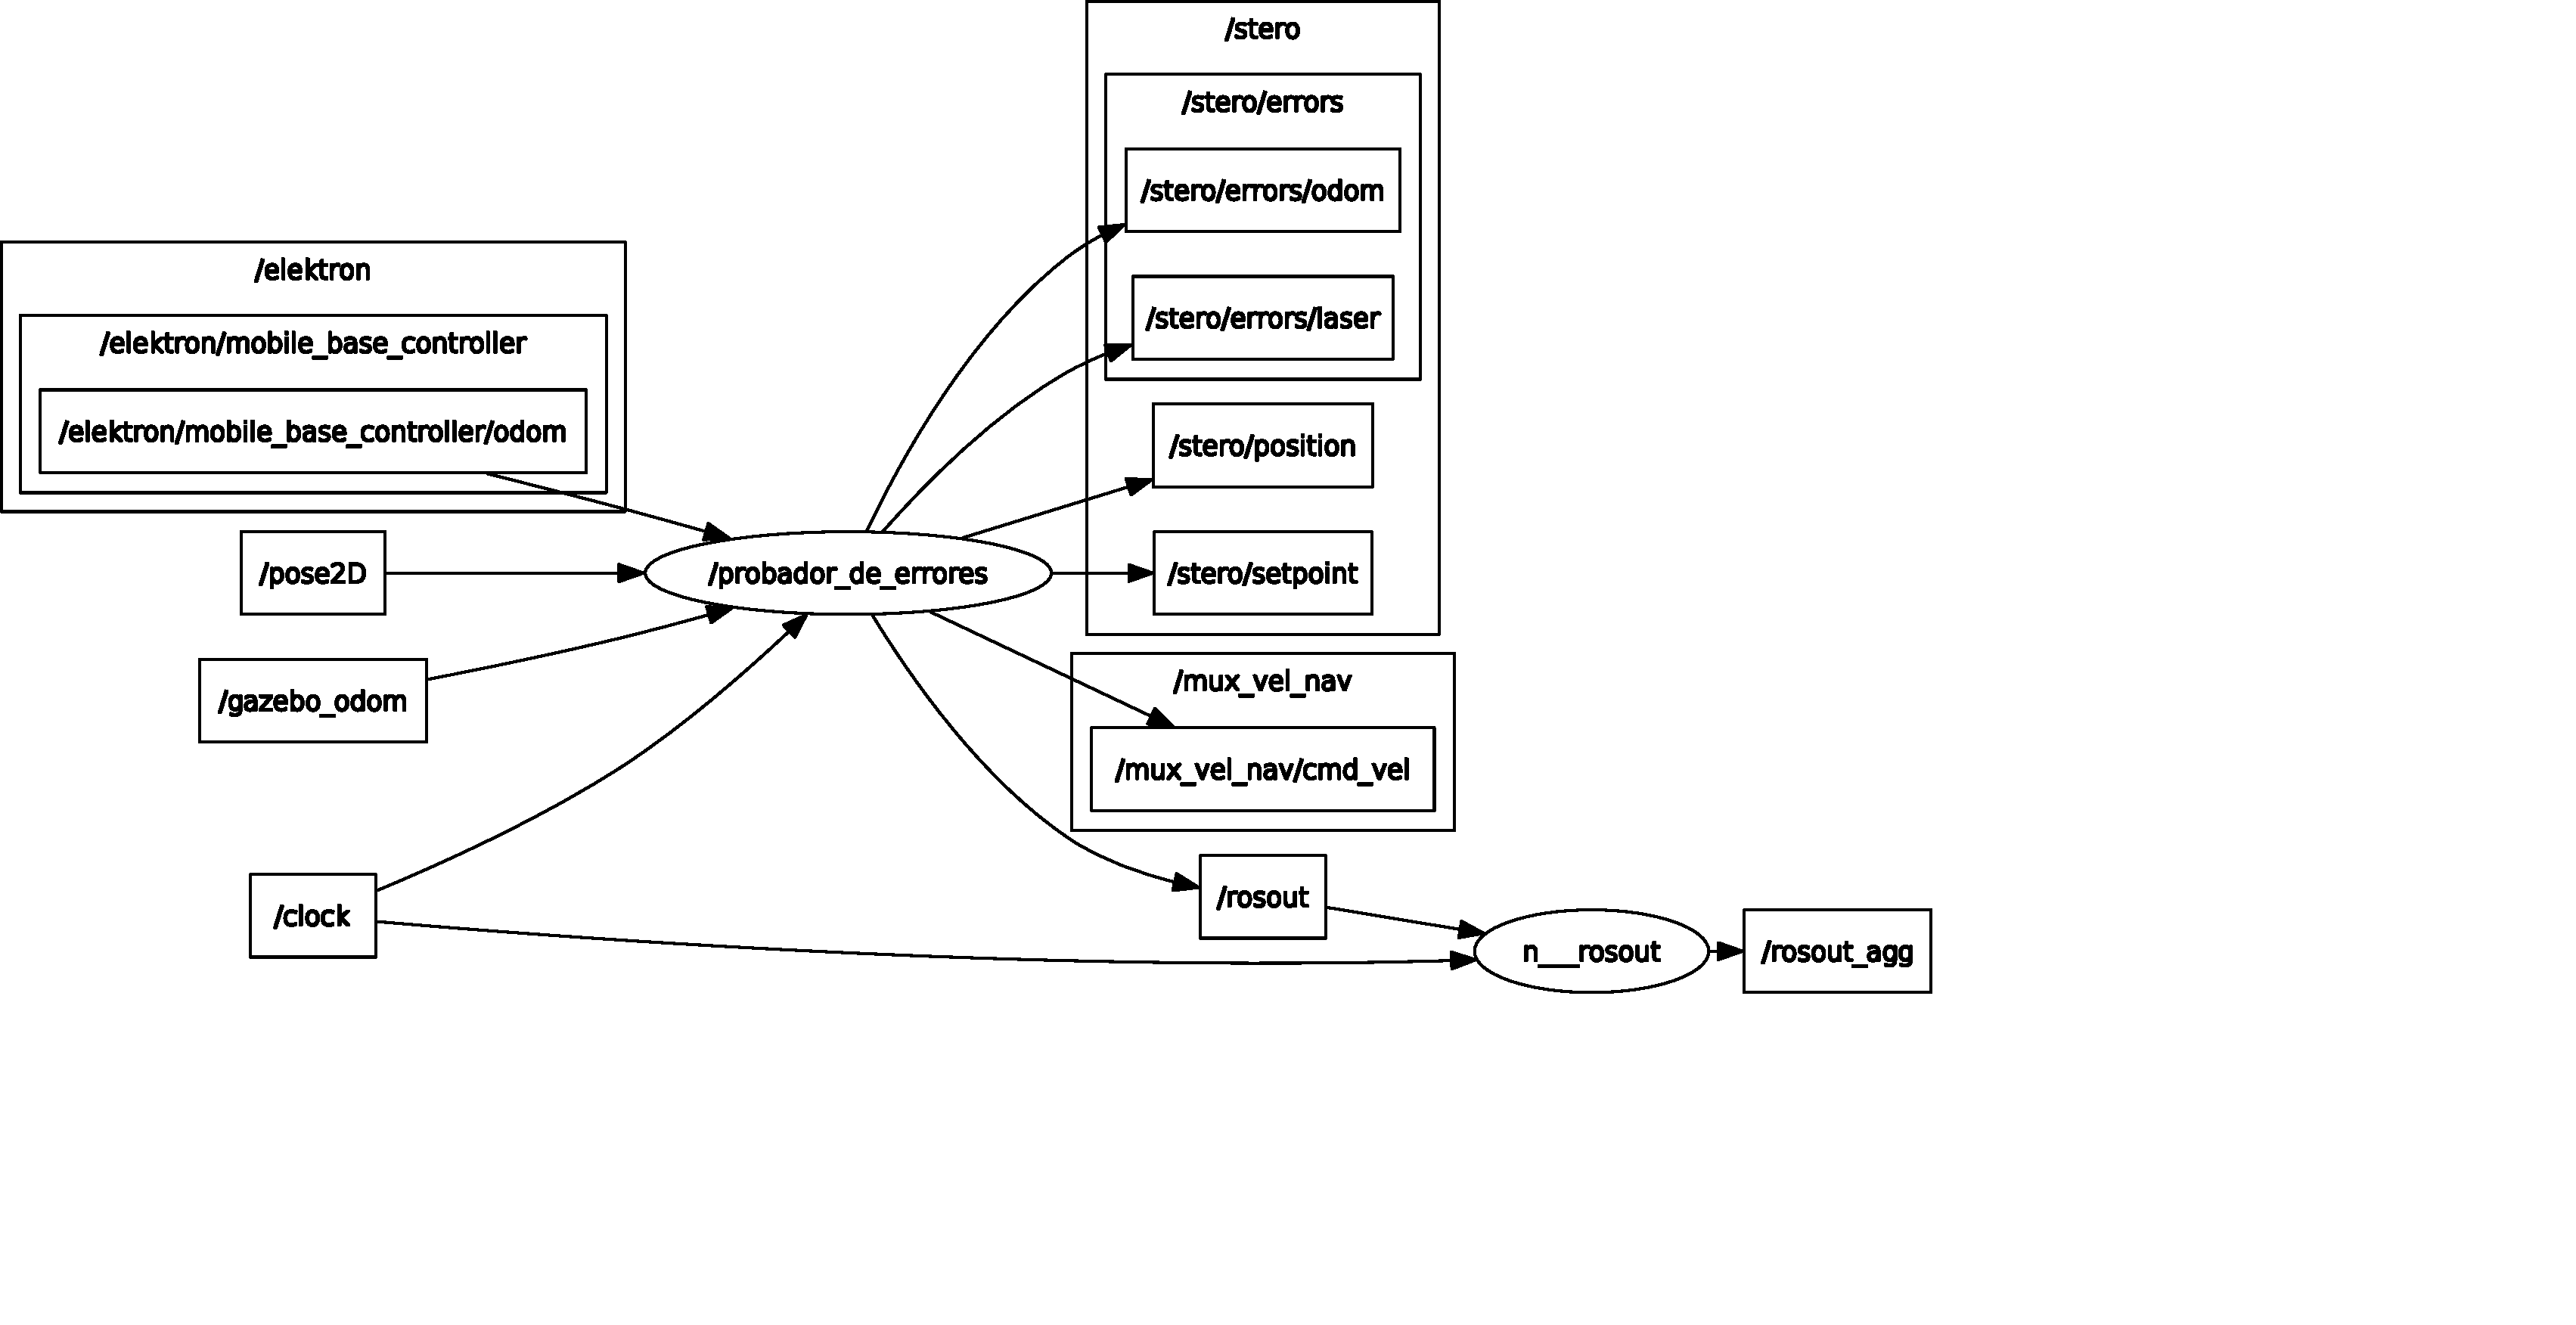
\includegraphics[scale=0.33]{./figures/pro1/pro1_system.pdf}
	\caption{Struktura systemu akwizycji danych z odometrii}
\end{figure}

Zgodnie z przyjętą konwencją nazewniczą, węzeł zajmujący się równocześnie akwizycją
i sterowanie robota został nazwany \texttt{probador\_{}de\_{}errores}. Uruchomienie 
skryptu powodowało pojawienie się następującego komunikatu:\\
\\
\texttt{Bienvenidos!}\\
\texttt{Sterowanie i Symulacja Robotow. Mini-projekt 3.}\\
\texttt{Wykonanie: Konrad Winnicki \& Jakub Sikora}\\
\texttt{Dostepne argumenty wywolania:}\\
\\
\texttt{-l, --line:                    test jazdy po linii}\\
\texttt{-c, --circle:                  test obrotu}\\
\texttt{-s, --square:                  test jazdy po kwadracie}\\


Ponowne uruchomienie programu z odpowiednim argumentem powodowało rozpoczęcie 
testu. Przed testem należało upewnić się że robot znajduje się w pozycji początkowej.

\section{Opis działania węzła zbierającego dane}
\label{pro1_datadescription}
Głównym zadaniem węzła była akwizycja danych z odometrii oraz publikacja danych.

\subsection{Subskrypcje tematów}
\label{pro1_datadescription_subscribers}

Węzeł jawnie subskrybował trzy tematy:

\begin{itemize}
	\item \texttt{/elekton/mobile\_{}base\_{}controller/odom} - temat z pozycją uzyskaną z enkoderów na kołach
	\item \texttt{/pose2D} - temat z pozycją uzyskaną z czujnika laserowego
	\item \texttt{/gazebo\_{}odom} - temat z pozycją referencyjną uzyskaną z symulatora\\
\end{itemize}

W węźle zaimplementowalismy funkcje reagujące na przyjście nowej wiadomości, które wyciągały 
interesujące nas dane i zapisywały je do globalnego stanu węzła. 

\subsection{Rozgłaszanie na temacie}
\label{pro1_datadescription_broadcasters}
Węzeł wysyła wiadomości na następujących tematach:
\begin{itemize}
	\item \texttt{/stero/errors/odom} - na tym temacie jest nadawany aktualny błąd odometrii z enkoderów
	wyliczony na podstawie referencyjnego pomiaru pozycji z tematu \texttt{gazebo\_{}odom}
	\item \texttt{/stero/errors/laser} - na tym temacie jest nadawany aktualny błąd odometrii z czujnika 
	laserowego wyliczony na podstawie referencyjnego pomiaru pozycji z tematu \texttt{gazebo\_{}odom}
	\item \texttt{/stero/position} - temat na której robot nadaje pozycję w której myśli że aktualnie jest,
	w zależności od wybranego sprzężenia (pozycja od enkoderów/pozycja z lasera)
	\item \texttt{/stero/setpoint} - temat z zadaną pozycją do której robot aktualnie dąży, ostatecznie 
	nie został wykorzystany w projekcie, zaimplementowany z powodu pierwotnego złego zrozumienia zadania\\
\end{itemize}

Co każdy obieg pętli sterującej robotem, system rozgłasza nowe wiadomości na wyżej wymienionych tematach.
Dzięki temu mogliśmy w prosty sposób za pomocą narzędzia \texttt{rosbag} nagrać wiadomości do późniejszej 
analizy.

\section{Opis działania węzła sterującego robota}
\label{pro1_controldescription}
Węzeł \texttt{probador\_{}de\_{}errores} zajmuje się również sterowaniem robota w ramach 
przeprowadzanego testu. Do wyboru są trzy testy: 

\begin{itemize}
	\item test jazdy na wprost
	\item test obrotu
	\item test jazdy po kwadracie\\
\end{itemize}

Każdy z testów przeprowadzany jest na zasadzie podobnej jak do tej przedstawionej w \ref{lab1_interpolation_noodom}.

\section{Sposób analizy danych}
\label{pro1_dataanalysis}
Po przeprowadzeniu testów, uzyskaliśmy bardzo dużo danych do analizy. Zdecydowaliśmy się na skorzystanie z 
z programu \textsc{Matlab}. Program oferuje możliwość instalacji pakietu \texttt{Robotics System Toolbox}, 
który posiada narzędzia do analizy danych zagregowanych w plikach \emph{.bag} z wyszczególnieniem poszczelnych 
tematów. W pierwszej kolejności należy stworzyć obiekt reprezentujący plik \emph{.bag} za pomocą polecenia 
\begin{center}
	\texttt{bag = rosbag(path\_{}to\_{}rosbag\_{}file)}
\end{center}

Korzystając z otrzymanego obiektu, możemy wyciągać podobiekty tematów na podstawie ich nazwy za pomocą następującego
polecenia
\begin{center}
	\mbox{\texttt{odom = select(bag,'Topic','/elektron/mobile\_{}base\_{}controller/odom')}}
\end{center}

Wykorzystując obiekt tematu, w prosty sposób można wyodrębnić obiektu typu \texttt{timeseries}, 
które w bardzo prosty sposób można przedstawiać na wykresach, dzięki temu że wiążą dyskretną wartość wyjścia
z dyskretnym czasem próbkowania. Obiekty te tworzymy za pomocą polecenia
\begin{center}
	\texttt{ts\_{}odom\_{}X = timeseries(odom, 'Pose.Pose.Position.X');}
\end{center}

Mając już obiekt typu \texttt{typeseries}, pozostało już tylko stworzyć wykres i zapisać go do dalszej analizy.
Wykres tworzymy za pomocą standardowego polecenia
\begin{center}
	\texttt{plot(ts\_{}odom\_{}X)}
\end{center}

Korzystając z wyżej wymienionych poleceń, udało nam się napisać skrypt \texttt{bag\_{}analyzer.m}, który
automatycznie generuje wykresy błędów i pozycji we wszystkich współrzędnych z podanego rosbaga.  

\section{Wykresy i wnioski}
\label{pro1_figures}

\subsection{Test jazdy na wprost}
\label{pro1_figures_line}

\begin{figure}[H]
	\centering
	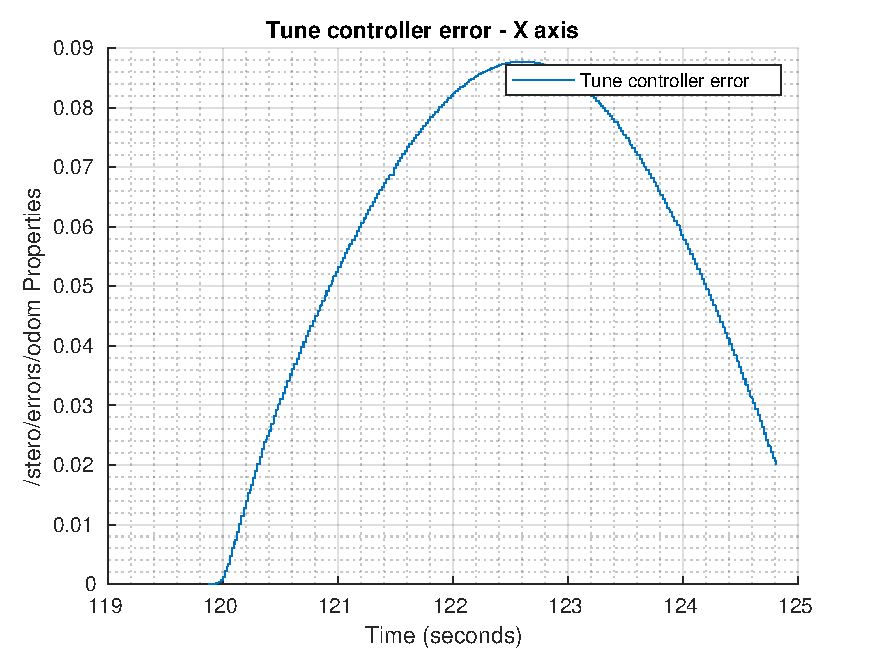
\includegraphics[scale=0.75]{./figures/pro1/line_tune/line_tune_x.pdf}
	\caption{Błąd odometrii we współrzędnej x przy sterowaniu za pomocą \texttt{tune\_{controller}} w teście jazdy na wprost}
\end{figure}

\begin{figure}[H]
	\centering
	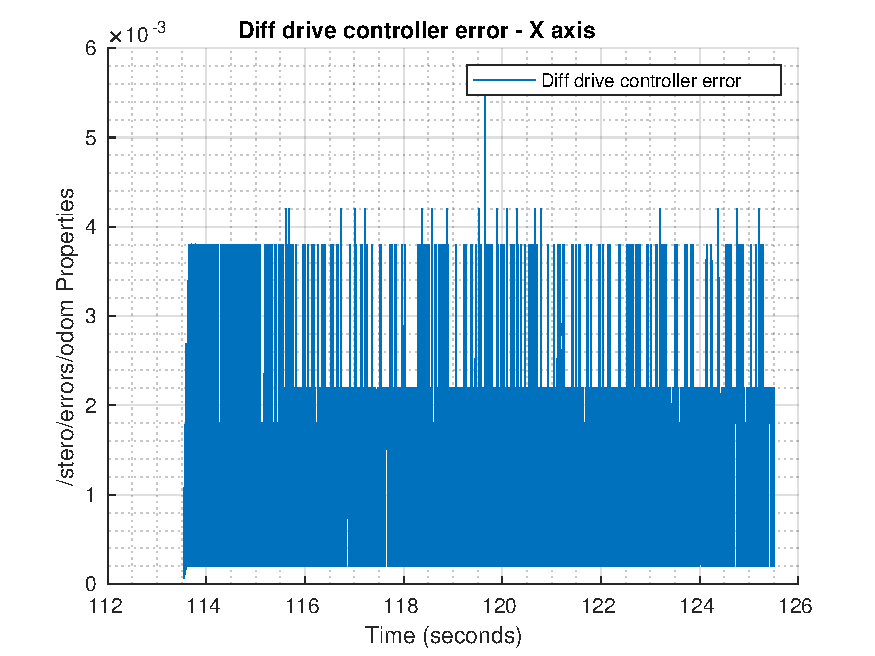
\includegraphics[scale=0.8]{./figures/pro1/line_diff/line_diff_x.pdf}
	\caption{Błąd odometrii we współrzędnej x przy sterowaniu za pomocą \texttt{diff\_{}drive\_{}controller} w teście jazdy na wprost}
\end{figure}

\begin{figure}[H]
	\centering
	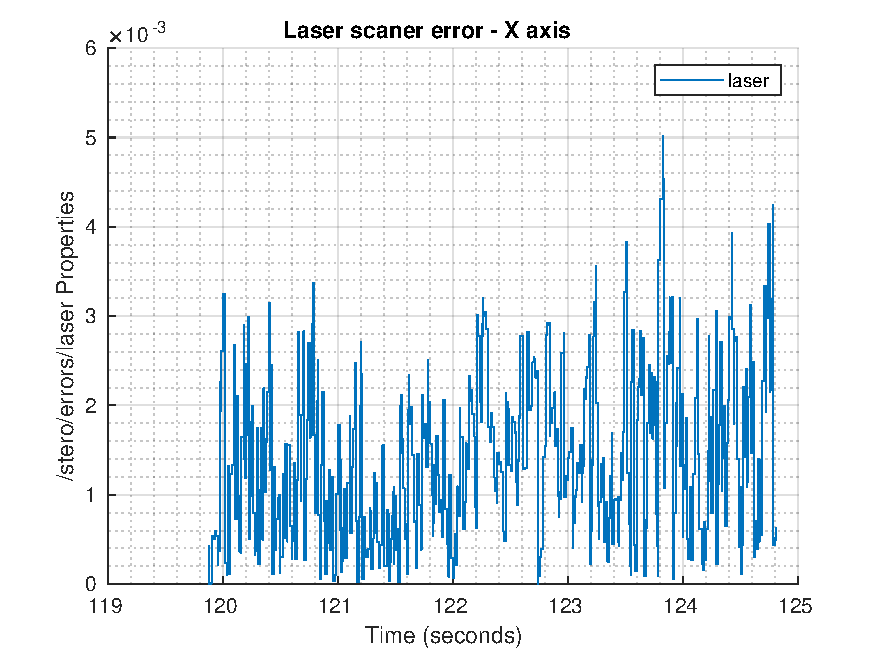
\includegraphics[scale=0.8]{./figures/pro1/line_tune/line_tune_laser_x.pdf}
	\caption{Błąd odometrii we współrzędnej x uzyskany z czujnika laserowego w teście jazdy na wprost}
\end{figure}

Na podstawie wyżej przedstawionych wykresów, można jednoznacznie stwierdzić że sterownik \texttt{tune\_{}controller} 
w trakcie szybkiej jazdy na wprost gubi pozycję, szczególnie w trakcie startowania. W trakcie zatrzymywania się, 
błąd zmalał. Mimo wszystko, błąd pozycji jest znaczny, szczególnie w porównaniu z błędami sterownika
\texttt{diff\_{}drive\_{}controller} i skanera laserowego. W trakcie jazdy na wprost, błędy drugiego sterownika i 
skanera laserowego pozostają na porównywalnym poziomie i są rzędu milimetrów. 

\newpage
\subsection{Test obrotu}
\label{pro1_figures_circle}

\begin{figure}[H]
	\centering
	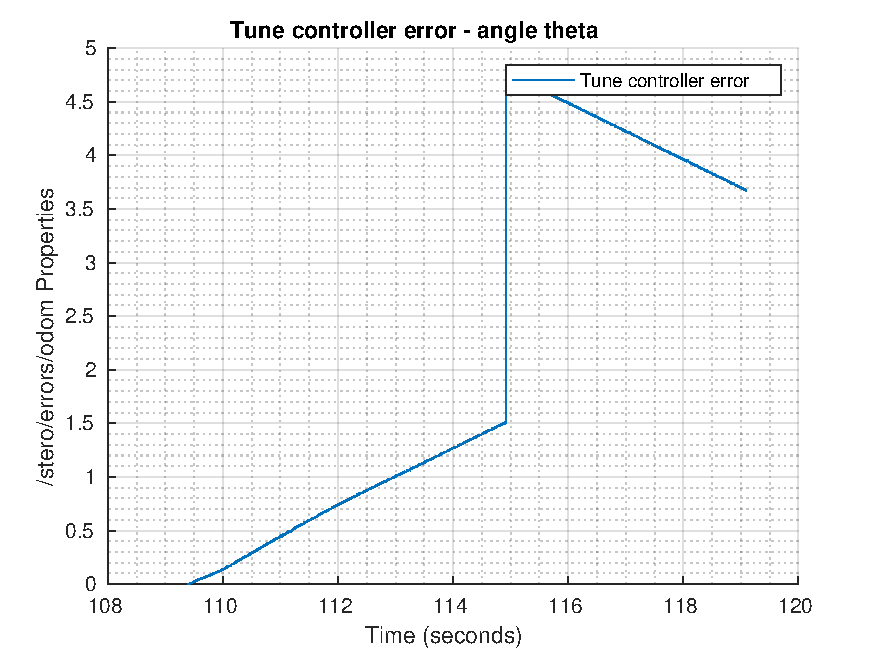
\includegraphics[scale=0.85]{./figures/pro1/circle_tune/circle_tune_theta.pdf}
	\caption{Błąd odometrii we współrzędnej $\theta$ przy sterowaniu za pomocą \texttt{tune\_{controller}} w teście obrotu}
\end{figure}

\begin{figure}[H]
	\centering
	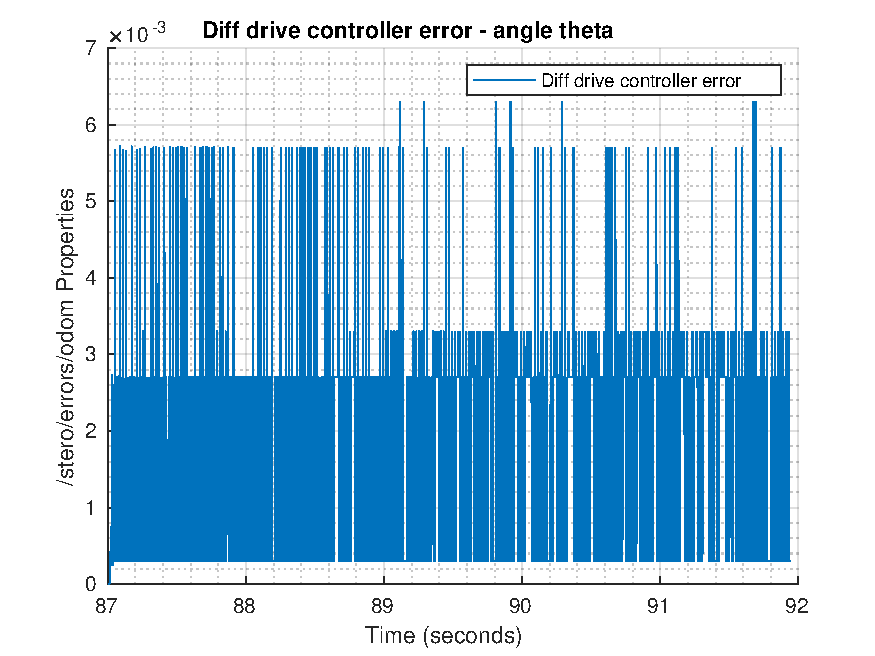
\includegraphics[scale=0.85]{./figures/pro1/circle_diff/circle_diff_theta.pdf}
	\caption{Błąd odometrii we współrzędnej $\theta$ przy sterowaniu za pomocą \texttt{diff\_{}drive\_{}controller} w teście obrotu}
\end{figure}
\newpage

\begin{figure}[H]
	\centering
	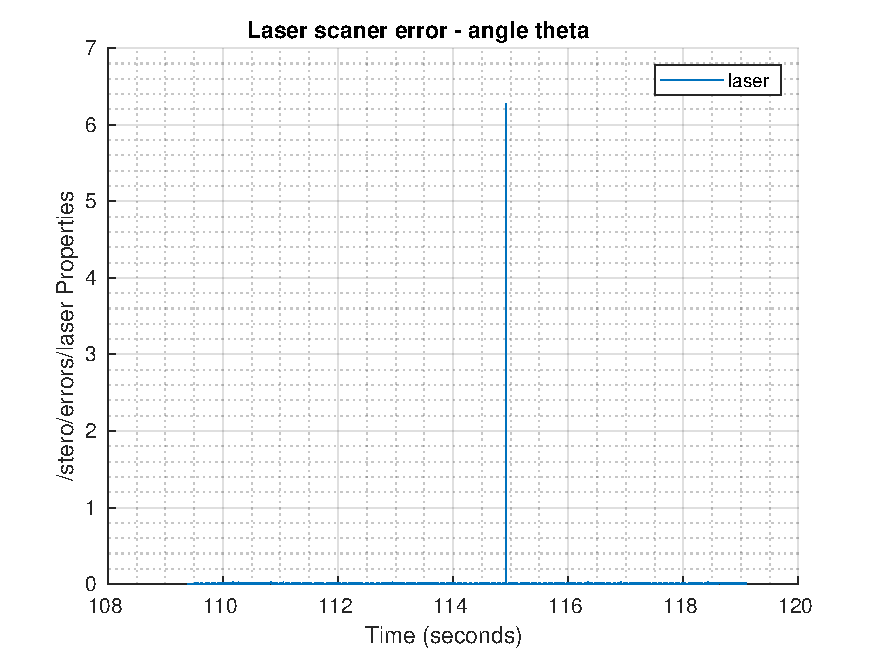
\includegraphics[scale=0.85]{./figures/pro1/circle_tune/circle_tune_laser_theta.pdf}
	\caption{Błąd odometrii we współrzędnej $\theta$ uzyskany z czujnika laserowego w teście obrotu}
\end{figure}

W przypadku testu obrotu, ponownie \texttt{tune\_{controller}} wypadł najsłabiej. W trakcie obracania się,
sterownik gubi kąt. Wynika to ze sposobu obracania się robota o bazie różnicowej. Pozostałe dwa sygnały utrzymują
się w granicach akceptowalnych błędów, oscylując około wartości co odpowiada $0,1719$ stopnia. Charakterystyczne piki
wynikają ze sposobu normalizacji kąta obrotu.
\newpage

\subsection{Test kwadratu}
\label{pro1_figures_square}
\subsubsection{\texttt{tune\_{}controller}}
\label{pro1_figures_square_tune}
\begin{figure}[H]
	\centering
	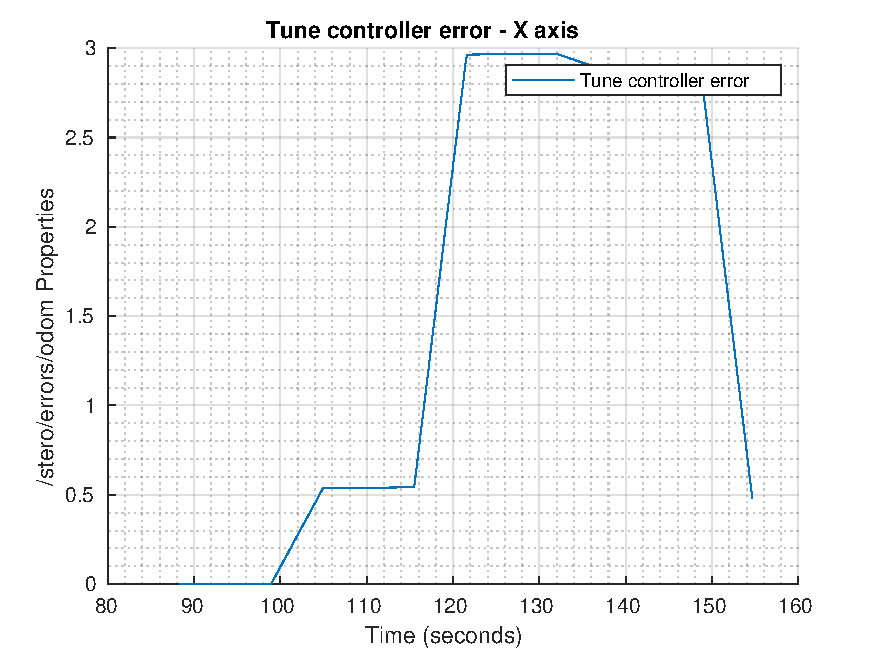
\includegraphics[scale=0.85]{./figures/pro1/square_tune/square_tune_x.pdf}
	\caption{Błąd odometrii we współrzędnej x przy sterowaniu za pomocą \texttt{tune\_{controller}} w teście kwadratu}
\end{figure}

\begin{figure}[H]
	\centering
	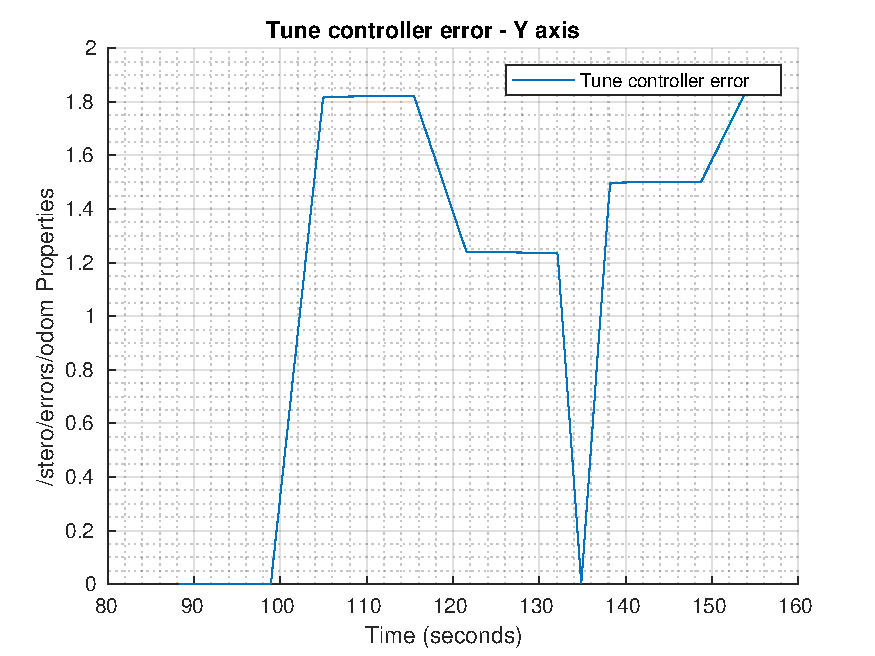
\includegraphics[scale=0.85]{./figures/pro1/square_tune/square_tune_y.pdf}
	\caption{Błąd odometrii we współrzędnej y przy sterowaniu za pomocą \texttt{tune\_{controller}} w teście kwadratu}
\end{figure}

\begin{figure}[H]
	\centering
	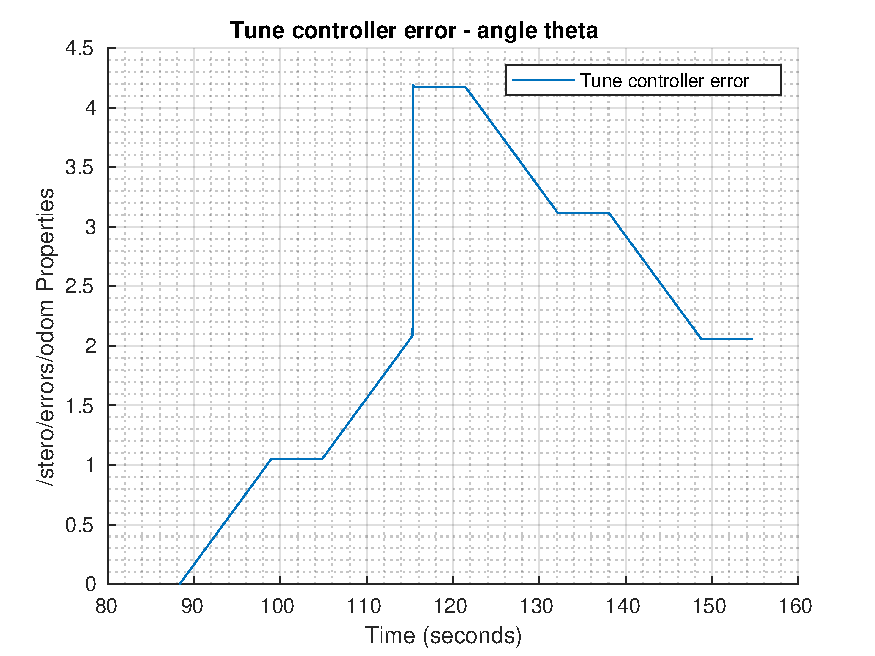
\includegraphics[scale=0.85]{./figures/pro1/square_tune/square_tune_theta.pdf}
	\caption{Błąd odometrii we współrzędnej $\theta$ przy sterowaniu za pomocą \texttt{tune\_{controller}} w teście kwadratu}
\end{figure}

\subsubsection{\texttt{diff\_{}drive\_{}controller}}
\label{pro1_figures_square_diff}
\begin{figure}[H]
	\centering
	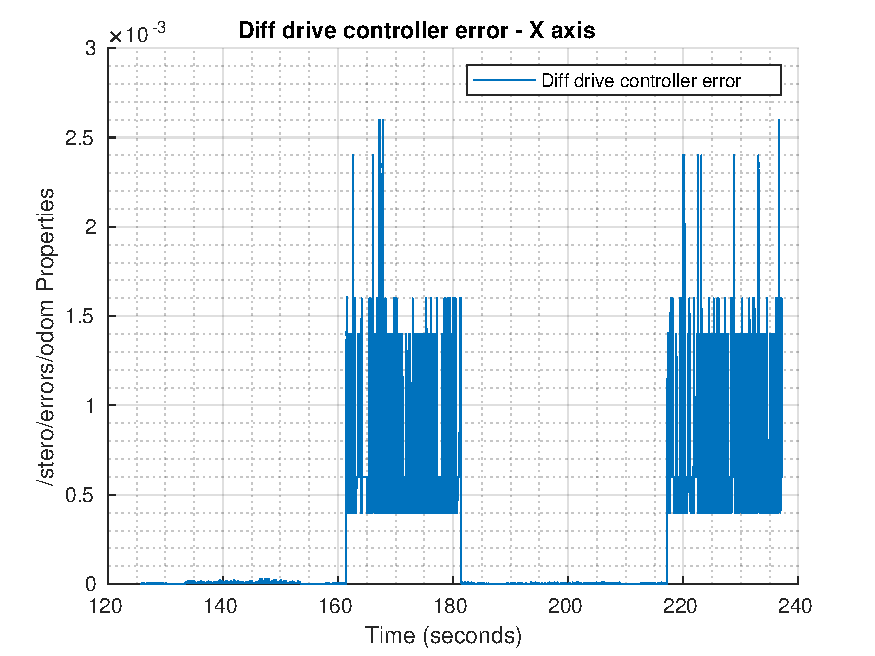
\includegraphics[scale=0.85]{./figures/pro1/square_diff/square_diff_x.pdf}
	\caption{Błąd odometrii we współrzędnej x przy sterowaniu za pomocą \texttt{diff\_{}drive\_{}controller} w teście obrotu}
\end{figure}

\begin{figure}[H]
	\centering
	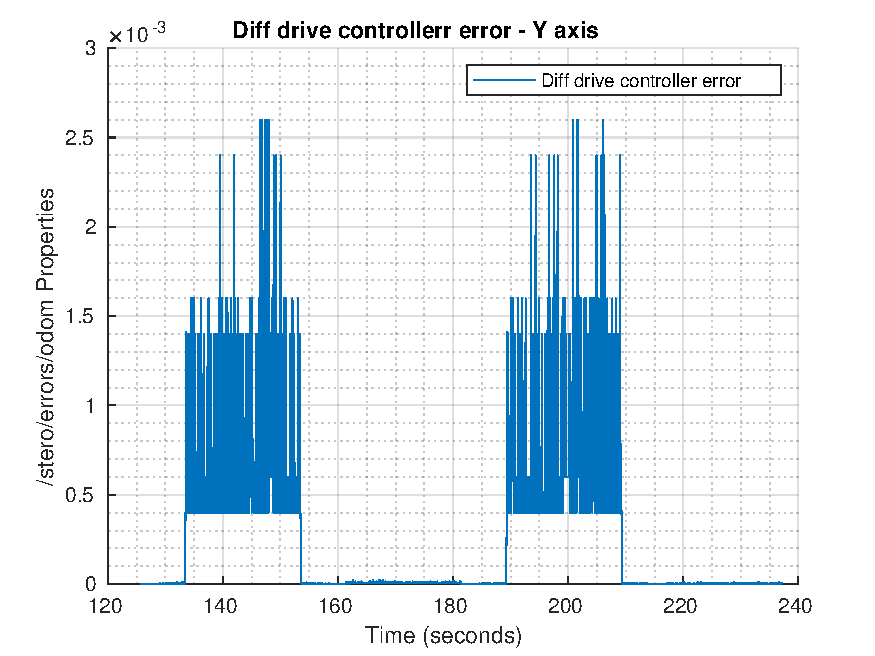
\includegraphics[scale=0.85]{./figures/pro1/square_diff/square_diff_y.pdf}
	\caption{Błąd odometrii we współrzędnej y przy sterowaniu za pomocą \texttt{diff\_{}drive\_{}controller} w teście obrotu}
\end{figure}

\begin{figure}[H]
	\centering
	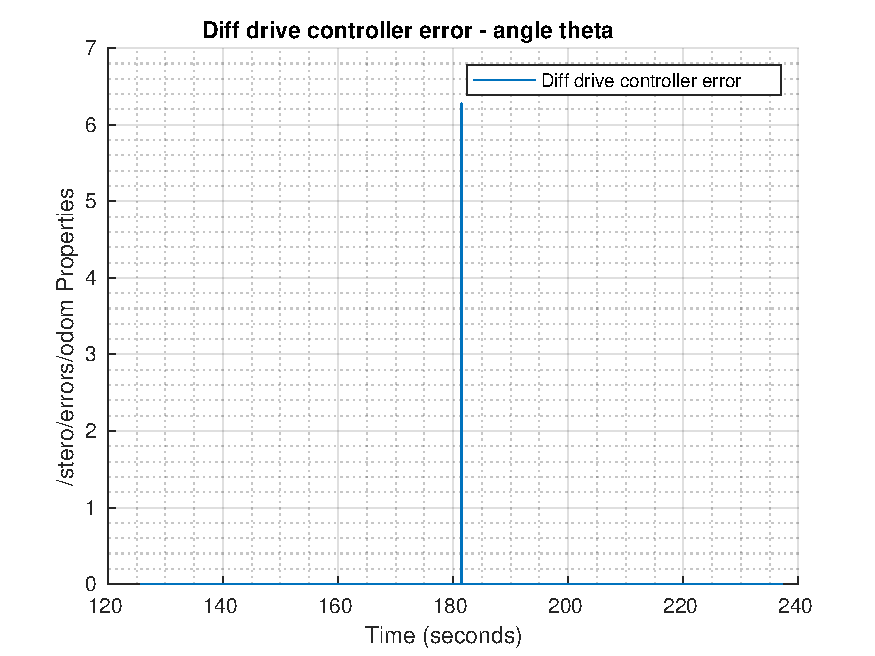
\includegraphics[scale=0.85]{./figures/pro1/square_diff/square_diff_theta.pdf}
	\caption{Błąd odometrii we współrzędnej $\theta$ przy sterowaniu za pomocą \texttt{diff\_{}drive\_{}controller} w teście obrotu}
\end{figure}

\subsubsection{\texttt{laser\_{}scan\_{}matcher}}
\label{pro1_figures_square_laser}
\begin{figure}[H]
	\centering
	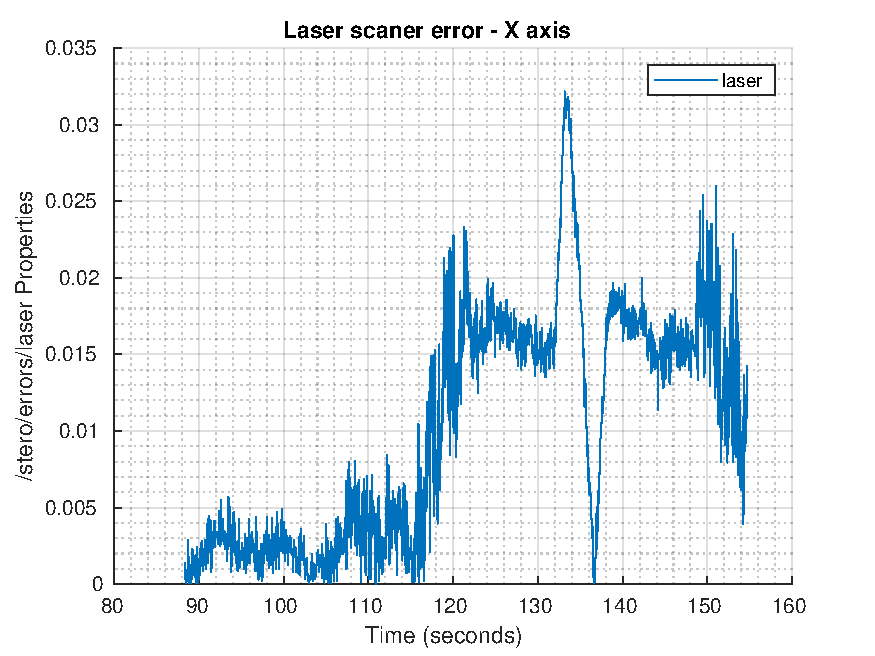
\includegraphics[scale=0.85]{./figures/pro1/square_tune/square_tune_laser_x.pdf}
	\caption{Błąd odometrii we współrzędnej x uzyskany z czujnika laserowego w teście kwadratu}
\end{figure}

\begin{figure}[H]
	\centering
	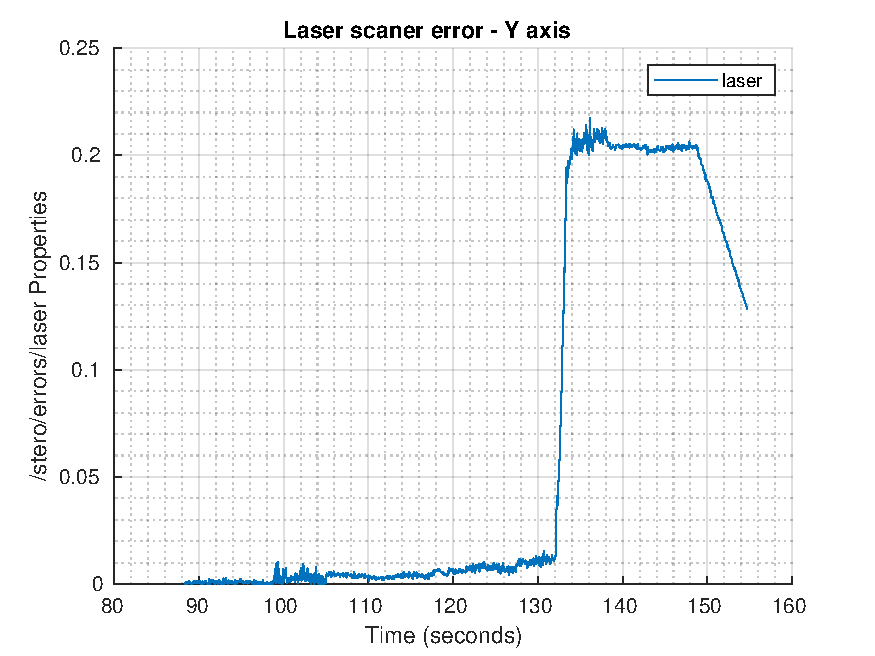
\includegraphics[scale=0.85]{./figures/pro1/square_tune/square_tune_laser_y.pdf}
	\caption{Błąd odometrii we współrzędnej y uzyskany z czujnika laserowego w teście kwadratu}
\end{figure}

\begin{figure}[H]
	\centering
	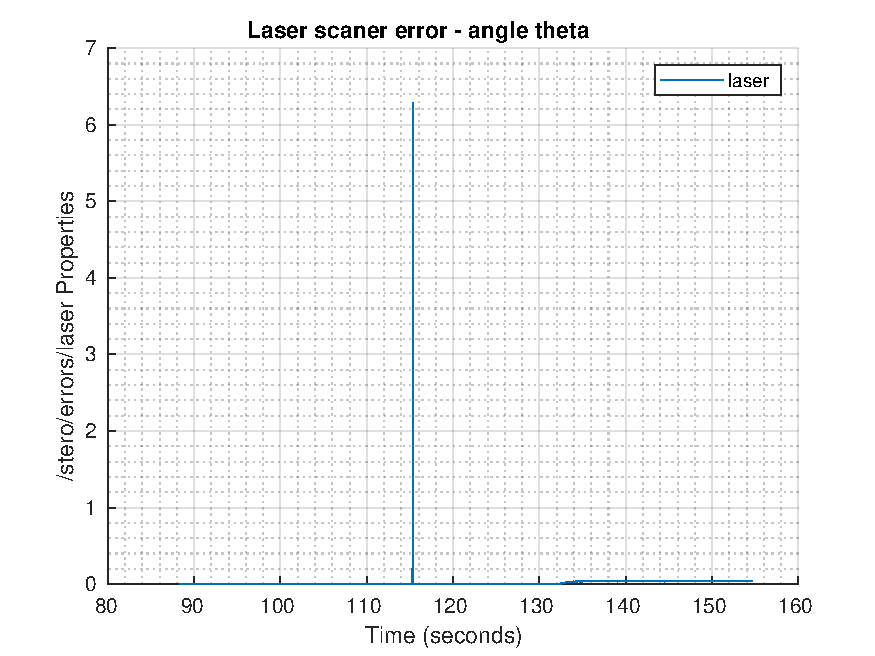
\includegraphics[scale=0.85]{./figures/pro1/square_tune/square_tune_laser_theta.pdf}
	\caption{Błąd odometrii we współrzędnej $\theta$ uzyskany z czujnika laserowego w teście kwadratu}
\end{figure}
\vspace{0.8cm}

\subsubsection{Wnioski}
Na podstawie wyżej przedstawionych wykresów można jednoznacznie stwierdzić że sterownik \texttt{diff\_{}drive\_{}controller}
jest zdecydowanie lepszy od sterownika \texttt{tune\_{}controller}. Dzieje się tak ponieważ sterownik
\texttt{tune\_{}controller} nie został odpowiednio dostrojony. Poprawę jakości odometrii z tego sterownika
można osiągnąć poprzez poprawienie konfiguracji parametrów, co zostało pozostawione ochotnikom (z racji 
że czas przed sesją jest niezwykle cennym surowcem, szczególnie na tym wydziale, tym razem wyjątkowo ochotnikami nie zostaliśmy).\\
\\
\indent{} Pomiary pozycji względnej za pomocą czujnika laserowego LIDAR uzyskują zaskakująco dobrą 
dokładność. Zmierzone błędy w złożonym zadaniu jazdy po kwadracie utrzymują się poniżej rozsądnego poziomu.
Duży skok błędu wzdłuż współrzędnej y wynika z tego że w tej osi nie było żadnych ścian w pobliżu robota,
co sprawiło że pomiar był mniej dokładny. Takie ściany robot miał przed sobą wzdłuż osi x, co pozwoliło na 
osiągnięcie znacznie mniejszych błędów. \\
\\
\indent{} W przypadku tak bogatej platformy jaką jest robot Elektron, najlepsze rezultaty możemy osiągnąć poprzez 
wsparcie sterownika \texttt{diff\_{}drive\_{}controller} pomiarami ze skanera laserowego. Połączenie 
danych z obu źródeł ma potencjał aby stać się źródłem bardzo dokładnego wskaźnika względnej pozycji, co 
jest kluczowe w skutecznym nawigowaniu robotem mobilnym o tak skomplikowanej bazie.



\chapter{Laboratorium 2}

\section{Stworzone środowisko i jego mapa}

\section{Przykładowe ścieżki zaplanowane w środowiskach}

\section{Pliki uruchomieniowe symulacji}


\chapter{Projekt 2}

\section{Struktura sterownika robota}

\section{Opis działania węzła planującego}

\section{Pliki konfiguracyjne map kosztów oraz lokalnego planera}

\section{Wyjaśnienie zastosowanych parametrów}
Dlaczego taki parametr ustawiono i dlaczego taka wartość?
\section{Weryfikacja działania}
Zrzuty ekranu z zaplanowaną i wykonaną ścieżką (Typ
wizualizacji: Odometry ): http://wiki.ros.org/rviz/DisplayTypes/Odometry
\end{document}